\chapter{Neural Networks and Deep Learning}
\label{C:background}

This chapter introduces neural network notation and concepts which will be used in later chapters.

\section{Introduction}

Since Krizhevsky et al.'s AlexNet \cite{alexnet} in 2012, an incredible number of problems are now being solved with the help Artificial Neural Networks (NN), including image classification, translation of natural language, speech encoding, autonomous driving, computer-generated art and more. Any particular NN is not designed but discovered by gradient descent, where the parameters of the NN are iteratively improved with respect to a loss function and a dataset, which together define the training objective that the NN will learn to achieve.

In this chapter, some notation will first be introduced and clarified so that it can be used later, and then an overview of the different aspects of neural networks will be given, such as different kinds of training objective.

\section{Notation}
\label{ss:dl-notation}

Many of the formalisms in deep learning rely on linear algebra. It is common to see tensors of rank 3 or higher in neural network implementations, along with scalars, vectors and matrices (ranks 0, 1 and 2 respectively). As a result, it is useful to have notation that clearly shows how functions may be applied across the various dimensions of these tensors.

First, a simple example using activation functions.

\subsection{Tensor index notation}

The ReLU activation function is defined as:
\begin{align}
\label{eqn:relu}
\begin{aligned}
    \fdef{\relu}{\R}{\R} \\
    \relu&(x) ≝ \max(0,x)
\end{aligned}
\end{align}
It is customary to use the symbol $\phi$ for activation functions. Activation functions are typically scalar functions, but are applied independently across all components of a tensor. This can be represented (and will be throughout) by the following notation -- for example, applying the ReLU activation function to a vector $\x$:
\begin{equation*}
\x'_i = \relu(\x_i)
\end{equation*}
In the above equation, the subscript $i$ shows that the function is applied \textit{independently} to each component of the vector $\x$.

This notation also works for multiple dimensions, including when an operation is not applied independently across some dimension. For example, the following is the \textit{softmax} function can be written, which is a vector valued function, applied independently across the rows of a $B\times N$ matrix $\X$ (which is used in the definition of the attention operation in \Cref{C:transformers}).

The softmax function is defined as:
\begin{equation}
\label{eqn:softmax}
\begin{split}
    \nvfdef{\sigma}{N}{N} \\
    \sigma(\x_n) ≝ \frac{e^{\x_{n}}}{\sum_{n'} e^{\x_{n'}}}
\end{split}
\end{equation}
The above function can be applied to a matrix $\X \in \R^{B\times N}$ independently over $B$ as follows:
\begin{align*}
\X'_{b,n} &= \sigma(\X_b)_{n} \\
          &= \frac{e^{\X_{b,n}}}{\sum_{n'} e^{\X_{b,n'}}}
\end{align*}

The term $\X_b$ refers to the $b$-th row of $X$ as a vector, as is common in tensor algebra software such as NumPy \cite{numpy} or TensorFlow \cite{tensorflow}. Here however the order of the subscript indices $b$ and $n$ is ignored -- the indices index their respectively-named dimensions. \textbf{This means that we abandon the distinction between row- and column-vectors}, and must therefore be explicit when representing matrix and vector products.

\subsection{Neural networks}

Some examples of basic neural network operations are given below, to clarify the notation further.

Let $N$ be the input dimensionality of a network, and $D$ the \textit{embedding} (or \textit{hidden} / \textit{latent}) dimensionality.  Let $\x \in \R^{N}$ be some input data embedded into an $N$-dimensional vector space. Let $W \in \R^{N \times D} $ be a matrix of learned weights, and let $\phi \colon \R \to \R$ be some non-linear function. Then, the computation done by one layer of a simple fully-connected neural network is represented as follows.
\begin{align}
\label{eqn:mlp}
\begin{aligned}
    f&_{\text{mlp}} \colon \R^N \to \R^D \\
    f&_{\text{mlp}}(\x) ≝ \phi(W\x) + \boldsymbol{b}
\end{aligned}
\end{align}
\begin{gather*}
    W \in \R^{N \times D}, \quad \vb \in \R^D
\end{gather*}
$W$ is the weight matrix, and $\vb$ is the bias vector, which together are the parameter set for this simple model. The output of the neural network is a $D$-dimensional vector.

A simple classifier network would be defined as follows, for $N$ dimensional data classified into $C$ classes, with $L$ hidden layers:
\begingroup
\allowdisplaybreaks
\begin{align*}
    \vfdef{f_0}{N}{D} \\
    f_{0}&(\x) = \phi(W_0 \x) + \vb &
    W_0 &\in \R^{N\times D} &
    \vb_0 &\in \R^{D}
\\ \\%
    \vfdef{f_\l}{D}{D} & \forall \l &\in 1,\dots,L \quad \\
    f_\l&(\x) = \phi(W_\l f_{\l-1}(\x)) + \vb_\l &
    W_\l &\in \R^{D\times D} \quad &
    \vb_\l &\in \R^{D}
\\ \\%
    \vfdef{f_L}{D}{C} \\
    f_{L}&(\x) = \sigma(W_L f_{L-1}(\x) + \vb_L) &
    W_L &\in \R^{D \times C} &
    \vb_L &\in \R^{C}
\\ \\%
    \vfdef{f_{\text{classifier}}}{N}{C} \\
    f_{\text{classifier}}& = f_L \circ f_{L-1} \circ \cdots \circ f_0 &
    \theta &= \rlap{\{$W_0, \cdots, W_L, \vb_0, \cdots, \vb_L \} $} \\ \numberthis \label{eqn:classifier}
\end{align*}
\endgroup
The parameters of the network are $\theta = \{W_0, ..., W_L, \vb_0, ..., \vb_{L}\}$. The output of the network is a $C$-dimensional vector, where each component is the probability that the input belongs to that class. This model would be trained with a categorical cross-entropy loss function -- which will be discussed in the next section.


\section{Tasks}
\label{s:tasks}

\begin{figure}
    \centering
        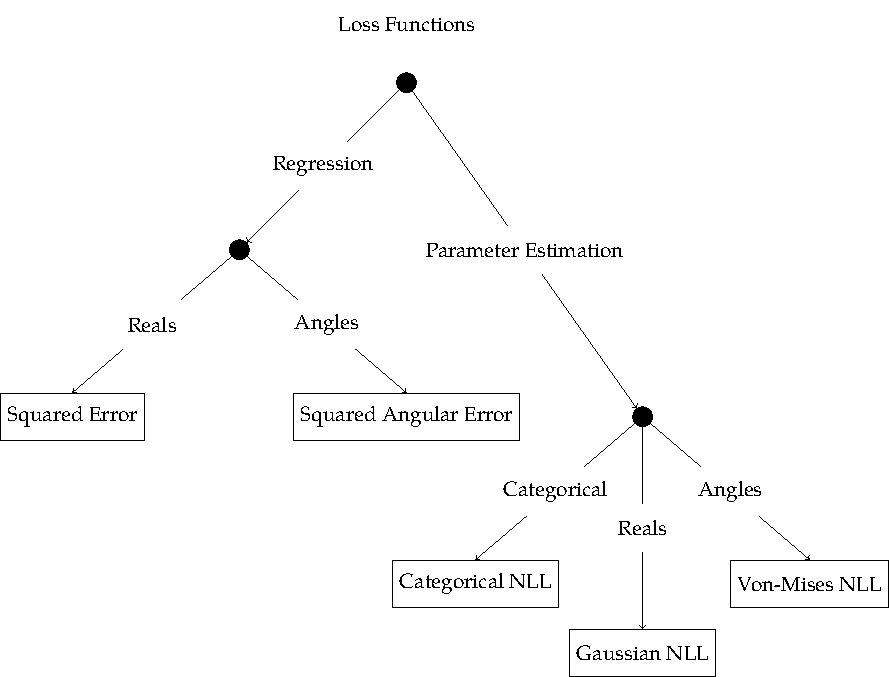
\includegraphics[width=.7\linewidth]{figures/ontology-1-loss.pdf}
        \vspace{1cm}
        \captionsetup{parskip=7pt}
        \captionof{figure}[Ontology of loss functions.]{We can split loss functions into two categories -- regression losses and parameter estimation losses.

        In the former, the loss function has the form of an error function. When minimizing this function, the model learns to output the expected value of the posterior $\E\left[p(y \mid x)\right]$ of the output $y$ given the input $x$. This is called a regression or maximum-a-posteriori (MAP) task.

        In the latter, the loss function has the form of a negative-log-likelihood (NLL) function. The model outputs the parameters of a probability distribution, and the loss function is the negative log-likelihood of the data under that distribution. This includes the case of categorical NLL (also called categorical cross-entropy), where the model outputs a probability distribution over a discrete set of classes.

        Models trained with a NLL loss learn to output an explicit posterior distribution $p(y \mid x)$, given a fixed functional form for $p$, such as a Gaussian, mixture of Gaussians, Categorical, Von-Mises, and many more. Depending on the task, and output format, different functional forms for $p$ may be appropriate.}
        \label{fig:ontology-loss}
\end{figure}

\begin{figure}
        \centering
        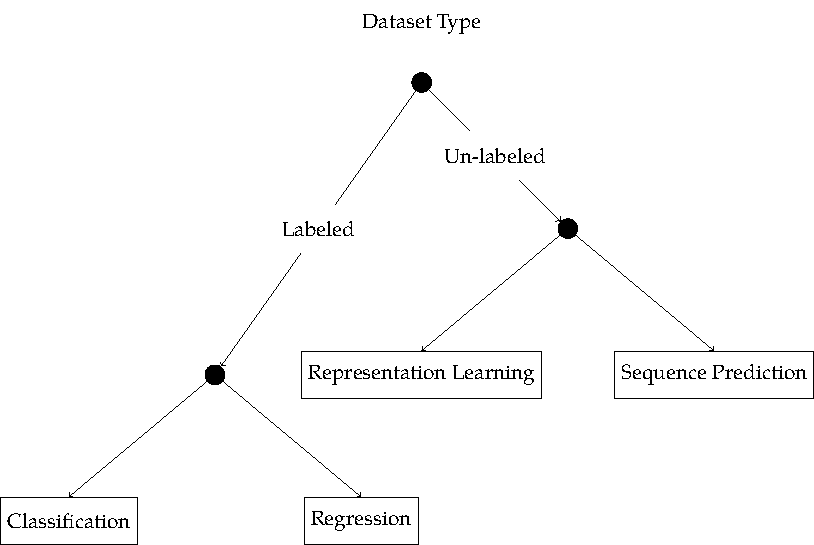
\includegraphics[width=.7\linewidth]{figures/ontology-2-task.pdf}
        \vspace{1cm}
        \captionsetup{parskip=7pt}
        \captionof{figure}[Ontology of dataset types]{
            Basic ontology of dataset types.

            When data is explicitly labeled a model can be trained on a task directly. However, the labeling process is often expensive, and in many cases, the data is unlabeled.

            When learning on unlabeled data, the goal is to learn a representation of the data that is useful for some downstream task.
        }
        \label{fig:ontology-task}
\end{figure}

\begin{figure}
        \centering
        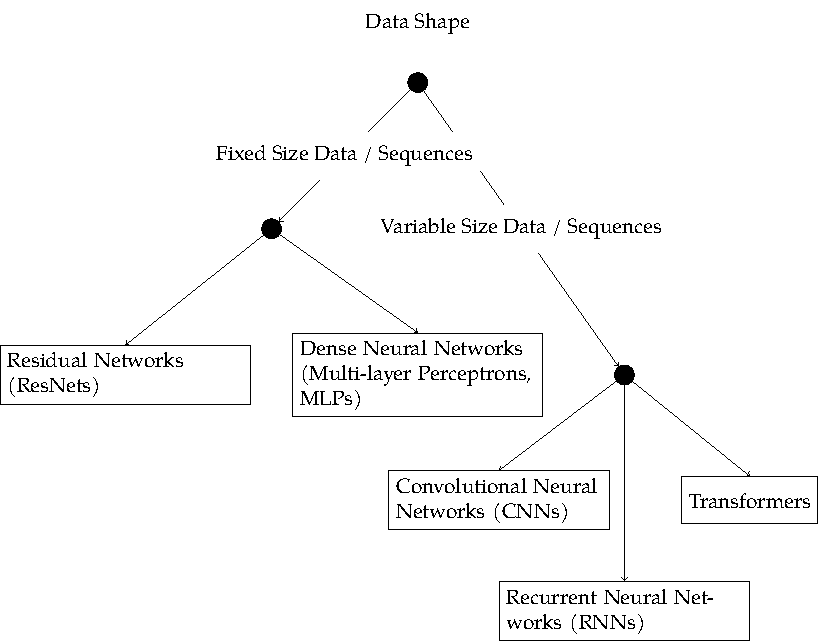
\includegraphics[width=.7\linewidth]{figures/ontology-3-input-shape.pdf}
        \vspace{1cm}
        \captionsetup{parskip=7pt}
        \captionof{figure}[Fixed vs variable input shape]{Neural network variants which support variable input shape.

        Due to their construction, MLPs and ResNets are restricted to a fixed input shape, and so can only be trained and used on data that is of a fixed size, such as tabular data, or data that has been processed into a fixed size by re-sampling, chunking etc.

        RNNs, CNNs and Transformers can accept variable length data, each with their own tradeoffs. They are typically more suitable for data that is naturally of variable size/length, such as text, audio or images.}
        \label{fig:ontology-input-shape}
\end{figure}


Neural networks are applied to a wide variety of tasks, such as classification of images, regression of time series data, prediction of tokenized language, and many more. The task that a neural network is applied to determines the loss function that is used to train the network, and the output format of the network. The input format / size / shape of the task also informs the choice of architecture of the neural network -- for example, a network that is trained on images will have a 2D input shape (which may be for fixed image sizes or variable image sizes), a network that is trained on tabular data will typically have a fixed-size input shape, and a time series model or language model will have a 1D variable-size input shape.

Different tasks lead to a number of different choices for the architecture and loss function. This section will contextualize the later work by giving a brief overview of the ways that different neural networks and training setups differ.

The following pages show some simple ontologies of the different considerations that combine to define a particular task and architecture, in particular:
\begin{enumerate}
    \item Training objective / loss function (\Cref{fig:ontology-loss})
    \item Data dimensionality / length (\Cref{fig:ontology-input-shape})
    \item Dataset format (\Cref{fig:ontology-task})
\end{enumerate}

\clearpage

The choice of training objective affects the settings in which a model can be used, which theoretical properties we get from it, and more. The structure of the data affects the type of model that can be used, and the format of the dataset affects what tasks we can learn from it.

\section{Deterministic models}

The simplest kind of training objective is regression. When we train a model with a regression objective it learns to predict the expected value of the output. Given input $x$, the model output $y = f(x)$ can be interpreted as $\E[p(y|x)]$. Regression is characterized by using an error function as the loss, for example \textit{mean-squared-error}.

\subsection{Mean squared error}
\label{ss:mse}

The squared error between two vectors $y$ and $\hat{y}$ is defined as
\newcommand{\se}{\mathcal{L}_{\text{SE}}}
\begin{align}
\label{eqn:se}
\begin{aligned}
    \fdef{\se}{\R^{D}×\R^{D}}{\R} \\
    \se&(y, \hat{y})_{i} ≝ \sum_i (y_{i} - \hat{y}_{i})^2
\end{aligned}
\end{align}
where $D$ is the dimensionality of the output vectors (which can simply be 1).
The error is the square of the euclidean distance between the two vectors.

More commonly in neural networks, the mean squared error is used, which is the average squared error over two batches/sequences of vectors $Y$ and $\hat{Y}$:
\newcommand{\mse}{\mathcal{L}_{\text{MSE}}}
\begin{align}
\label{eqn:mse}
\begin{aligned}
    \fdef{\mse}{\R^{N×D}×\R^{N×D}}{\R} \\
    \mse&(Y, \hat{Y}) ≝ \frac{1}{N} \sum_n \left[ \sum_i (Y_{ni} - \hat{Y}_{ni})^2 \right]
\end{aligned}
\end{align}
where $N$ is the number of samples in the batch.

This function sums the error over the \textit{feature} dimension $D$ and averages the error over the \textit{batch} dimension $N$. Averaging has no effect on the optimization -- it is simply that dividing by the batch and/or sequence length means that the loss value remains in the same range independent of the batch size or sequence length.

\section{Probabilistic models}

When modeling data, it is often useful to have a \textit{probabilitic} model of the data, rather than a deterministic model. This allows the model to quantify uncertainty about the model outputs, produce multiple different samples, and avoid problems when the output distribution is multi-modal.

To make a model probabilistic, we train it on a parameter-estimation task. This means the model now outputs the parameters of a probability distribution, and the loss function used corresponds to the functional form of that distribution. This is straightforward for scalar outputs, but when the data being modeled is high-dimensional, probabilistic models often become computationally expensive or intractable, and some different techniques or assumptions must be made.

There are a few common distributions used when training probabilistic models, such as the Gaussian, Categorical, and Logistic distributions.

\subsection{Categorical distribution}
\label{ss:cat-dist}

The most common probability distribution used in neural networks is the categorical distribution, which is used when a task involves predicting discrete variables, commonly classification. The distribution and corresponding loss function are defined as follows
\newcommand{\cat}{p_{\text{Cat}}}
\newcommand{\catloss}{L_{\text{Cat}}}
\begin{align}
\label{eqn:cat-dist}
\begin{aligned}
    \fdef{\cat}{\R^{C}}{\R} \\
    \cat&(x = i \mid \theta) ≝ \frac{e^{\theta_{i}}}{\sum_j \exp(\theta_{j})}
\end{aligned}
\end{align}
\begin{align}
\label{eqn:cat-loss}
\begin{aligned}
    \fdef{\catloss}{\R^{N×D}×\R^{N×D}}{\R} \\
    \catloss&(y, \hat{\theta}) ≝ \frac{1}{N} \sum_n -\log \cat (y_n \mid \hat{\theta}_n)
\end{aligned}
\end{align}
where $C$ is the number of classes, and $\theta$ are the parameters, and $N$ is the batch size. The equations are written in terms of unnormalized $\theta$ (called \textit{logits}), because it is common to implement it this way for better numerical stability with floating point numbers. The categorical distribution is also called the discrete distribution, and the loss function above is equivalent to the ``categorical cross-entropy'' loss.

\subsection{Gaussian distribution}
\label{ss:gauss-dist}

Another common distribution to use in parameter estimation is the Gaussian distribution, which is used for continuous variables with unbounded domain (eg. \cite{gaussian}). The distribution and corresponding loss function are defined as follows
\newcommand{\gauss}{p_{\text{Gauss}}}
\newcommand{\gaussloss}{L_{\text{Gauss}}}
\begin{align}
\label{eqn:gaussian-dist}
\begin{aligned}
    \fdef{\gauss}{\R^{D}×\R^{D}}{\R} \\
    \gauss&(x \mid \mu, \sigma) ≝ \frac{1}{\sqrt{2\pi\sigma^2}} \exp\left(-\frac{(x - \mu)^2}{2\sigma^2}\right)
\end{aligned}
\end{align}
\begin{align}
\label{eqn:gaussian-nll}
\begin{aligned}
    \fdef{\gaussloss}{\R×\R×\R}{\R} \\
    \gaussloss&(y, \hat{\mu}, \hat{\sigma}) ≝ \frac{1}{N} \sum_n - \log \gauss(y \mid \hat{\mu}_{n}, \hat{\sigma}_{n})
\end{aligned}
\end{align}
where $\mu$ and $\sigma$ are mean and variance parameters, and $N$ is the batch size. The Gaussian distribution is a continuous distribution, and so the loss function is the mean-squared-error loss.

\subsection{von-Mises distribution}
\label{ss:von-mises}

The von-Mises distribution (eg. \cite{von-mises}), also known as the circular normal distribution or Tikhonov distribution, is a distribution over angles on the unit circle. It is defined as follows:
\newcommand{\vm}{\text{vM}}
\begin{align}
\label{eqn:von-mises}
\begin{aligned}
    \fdef{\vm}{\R×\R}{\R} \\
    \vm&(\mu, \kappa) = \frac{1}{2\pi I_0(\kappa)} \exp(\kappa \cos(\theta - \mu))
\end{aligned}
\end{align}
where $\mu$ is the modal angle and the circular mean of the distribution, and $\kappa$ is a concentration parameter. The distribution is the uniform distribution on the circle when $\kappa = 0$, and becomes more concentrated as $\kappa$ increases.

We will use this definition later in \Cref{ss:amse-motivation}. 

$I_0$ is the modified Bessel function of the first kind of order zero:
\begin{align}
    \label{notation:bessel}
    \begin{aligned}
        \fdef{I_0}{\R}{\R} \\
        I_0&(x) ≝ \int_{-\pi}^\pi \exp(x \cos t) \, dt
    \end{aligned}
\end{align}

\section{Probabilistic models over high-dimensional data}

Let us imagine we are modeling a sequence of $N$ observations $\x_i \in \R^D$, $1 ≤ i ≤ N$ (each observation is a $D$-dimensional vector). To represent the joint distribution over this data, even with a simple gaussian distribution requires $DN + (DN)^2$ parameters ($DN$ means, plus a $DN \times DN$ covariance matrix). If $N$ is large, this is a very large number of parameters, but still manageable.

A gaussian however is limited in its ability to model the data. For example, it cannot model multi-modal distributions. To model multi-modal distributions, we could use a mixture of gaussians, but this increases the number of parameters even further, to $(DN + (DN)^2)K + K$, where $K$ is the number of mixture components, making sampling and inference much more expensive.

In general, the more expressive the family of distributions we use to model the data, the more parameters we need to represent the distribution and the more expensive it is to sample from the distribution.

There are a few main approaches to address this problem:
\begin{itemize}
    \item Discretization
    \item Independence assumptions
    \item Auto-regressive factorization
\end{itemize}

\subsection{Discretization}

One approach to managing the intractability of high-dimensional data is to discretize the data, and then model it with a categorical distribution. For example, we can use a clustering algorithm to learn a series of $K$ points within our $DN$-dimensional space, and then form a discrete distribution over these points. A discrete distribution over $K$ points has $K-1$ free parameters, so this approach reduces the number of parameters from $(DN)^2$ to $K-1$, and makes sampling and inference more efficient. However the discretization changes the domain of the data, which may not always be useful. Additionally, the larger the domain, the more cluster points we need to use, and we might not be able to find a good clustering of the data.

\subsection{Independence assumptions}

Independence assumptions are another way to reduce the number of parameters. For example, we could assume that the observations $\x_i$ are independent, and then model the sequence as a product of $N$ independent $D$-dimensional distributions. For a Gaussian, this means fixing parts of the co-variance matrix, and we often reduce to having a single variance parameter. A single variance parameter reduces the number of parameters from $(DN)^2$ to $DN$, but it also makes the model less expressive. For sequence data, this assumption is almost never valid along the sequence dimension, so this approach is not very useful.

\subsection{Auto-regressive factorization}
\label{ss:ar-factorization}

Auto-regressive factorization is a third approach to reducing the number of parameters. In this approach, we break down the joint distribution over the sequence into a product of conditional distributions, where each conditional distribution depends only on the previous observations. We then typically model all of these conditional distributions with the same model.

\begin{align}
    \label{eqn:ar-factorization}
    \begin{aligned}
        p(\x_1, \x_2, \ldots, \x_N) &= \prod_i^N p(\x_i | \x_1, \ldots, \x_{i-1}) \\
        &= p(\x_1) p(\x_2 | \x_1) p(\x_3 | \x_1, \x_2) \ldots p(\x_N | \x_1, \ldots, \x_{N-1})
    \end{aligned}
\end{align}

When we use an auto-regressive model to predict sequences, we usually choose some fixed order for this decomposition. For data with a temporal dimension, this is usually first-to-last, which is usually natural because the real process that generated the data had a causal structure in the temporal dimension.

However, it is valid to perform the decomposition in any order, for example choosing a random permutation of the sequence(s), with indices $J$ being the integers up to $N$ as above, but in an arbitrary order:
\begin{align}
    \label{eqn:ar-factorization-random}
    \begin{aligned}
        J &= [5, 3, 9, 1, ...] \\
        p(\x_5, \x_3, \ldots, \x_{J_N}) &= p(\x_5) p(\x_3 | \x_5) p(\x_9 | \x_5, \x_3) \ldots p(\x_{J_N} | \x_5, \x_3, \x_9, \ldots, \x_{J_{N-1}}).
    \end{aligned}
\end{align}
We can see that due to the product rule of probabilities $p(A, B)=p(A|B)P(B)$ that such a factorization will be correct regardless of the order of $J$.

In the case of data that does not have a temporal dimension, such as pixels in an image, or joint angles of a hand (within one frame), simple ordering may not always be the best. Also, some data may have very long sequences and latency requirements (such as character animation data), where it is expensive to generate the data in order, and we would instead like to generate only particular parts of the sequence.
